\chapter{Method}
\label{ch:method}
From the beginning it was clear that we want to apply convolution neural networks to spectrogram input. How this could be achieved and which techniques were applied is covered in this chapter.

\section{Machine learning}
\Gls{ml} is a fast evolving software art based on statistics as well as data and computer science. It is a subdivision of \gls{ai} where computer systems run statistical algorithmic models to effectively perform specific tasks without using explicit instructions by a human expert. Instead, they are recognize and learn patterns from the data they see.
More recently, \gls{ml} models were able to master tasks that were thought to be too complex for machines, combined with the ability to perform a given task consistently and tirelessly, they could speed up the experimental process enormously and enable much broader searches for patterns. Even more exciting is the finding that in some cases, computers seem to be able to learn patters that are beyond human perception.
\Gls{ml} is now used in many fields and plays a central role in tasks such as speech recognition and translation between languages, autonomous navigation of vehicles and article recommendations.

Adapting \gls{ml} to our problem results in applying a \gls{ml} algorithm to a set of data (our recordings) and some knowledge about this data (the syllable type with their time boundaries). Through learning from the training data, the algorithm can apply what it has learned to make a prediction about the type of the syllable exhibited in a given spectrogram. The algorithm is considered to have learnt the task, when more test samples are diagnosed as the correct syllable type as a result of optimizing its parameters.
As soon as the parameter change in a learning cycle does not result in a significant impact in performance, the \gls{ml} algorithm can be seen as stable.

\section{Pipeline}
In the context of ML, the pipeline is a set of components describing the fate of the data.
It starts at the creation of the data and ends in analysing the performance of the \gls{ml} algorithm.

\begin{figure}[H]
\centering
  \includegraphics[width=0.9\textwidth]{plot/pipeline.pdf}
  \caption{Flow diagram of the data pipeline adapted for this project. It shows the different formats into which the data is transformed, finally it is transformed in such a way that the \gls{ml} model can understand and process it.}
  \label{fig:pipeline}
\end{figure}

\section{Data preprocessing}
Data preprocessing defines all the processing and transformations which are applied to the data before it reaches its final form that can be digested by the \gls{ml} algorithm.
Certain concepts used for data preprocessing in this project are explained below.

\subsection{Silent detection}\label{sec:silent_detection}
For noise reduction and padding of the extracted audio parts containing the syllable, we had to extract background noise from the audios.

Adapted from the librosa.effect.split \cite{McFee2020Librosa.effects.splitDocumentation}, we detect silent parts based on the \gls{rms} energy of the audio. We set the threshold to the average of the \gls{rms} energy of the audio without the syllable parts in it, as these are known foreground parts.
This leads to a conservative definition of the background audio, as this method was originally intended only for padding and thus a low-noise background audio was the goal.
The entire algorithm unfolds as follows:

\begin{equation}\label{eq:silent_detection_1}
silent = \begin{cases} 1 & mse < mean(mse \text{ without label})+1, \\ 0 & \text{otherwise}. \end{cases}
\end{equation}
\begin{itemize}
    \item As shown in \ref{eq:silent_detection_1}, the samples belonging to silent are marked with 1 in the first step and then successive samples are composed into silent slices.
    \item The silent slices are then shrunk on both sides by \SI{5}{\milli\second} and filtered against a minimum length of 10 samples. The idea behind this (which is not proven to be true for every case) is to remove the samples in the slice, where the energy becomes stronger and could lead in concatenated slices to small peaks at the beginning and end of a slice.
    \item Finally, all silent slices that overlap with a label are filtered out.
\end{itemize}
\begin{figure}[H]
\centering
  \includesvg[inkscapelatex=false,width=0.9\textwidth]{image/generated/silent_detection_sample1.svg}
  \caption{Plot of the result of the silence detection algorithm. The blackcurrant rectangles are the silent parts, on both sides the piece of \SI{5}{\milli\second} by which the silent parts were reduced is shown in transparent light blue. The yellow rectangle is a labelling part.}
  \label{fig:silent_detection_sample1}
\end{figure}

\subsection{Audio splitting algorithm}\label{sec:splitting_algorithm}
For the second experiment, with the goal of finding and classifying syllable types in an audio recording of the bats, we additionally train the network to distinguish between syllables and background.
In a comprehensive approach, we would train the network to learn the beginning and end of syllables, similar to the problems in human handwriting recognition.
Since we do not have enough knowledge in this area for this work, as well as too little capacity to learn this, we have opted for a simple version where we include background patterns in the dataset and nothing more.
For the training dataset, therefore, a preprocessing step is to split the audio and label the resulting chunks as background or as the corresponding syllable contained in the chunk.
% For analyzing a audio file containing multiple different syllable, we adapted a moving window algorithm.
This is achieved by applying a moving window to the audio source and assigning the resulting audio slices to either the corresponding syllable type or the background.
The audio slice is assigned to the corresponding syllable type as soon as a defined percentage or more of a slice is covered by a syllable or the boundaries of the syllable lie within the window, see \figref{moving_window}.

\begin{figure}[H]
\centering
  \includesvg[inkscapelatex=false,width=0.9\textwidth]{image/generated/moving_window.svg}
  \caption{Visualisation of the audio splitting algorithm with a spectrogram as background from a labelled audio file. The rectangle with the purple borders represents the moving window with the assigned labels on the upper x-axes. The yellow rectangle covers the boundaries of the annotated syllable. For visualisation reasons, we used parameters (\SI{30}{\milli\second} window length and \SI{34}{\milli\second} strides) that do not result in overlapping windows.}
  \label{fig:moving_window}
\end{figure}

For the training dataset, in order to reduce the number of slices marked as background, we discarded them after successive background slices reached three times the window length.
Ideally, this should also prevent unlabelled syllables from being marked as background, as this concept ignores slices which are a bit further away from the labels.
In the hope that there are no unlabelled syllables near labelled syllables.

\subsection{Spectrogram}
For audio analysis, the Fourier transform is one of the main tools to depict the audio and understand its inner parts. In our digital world the \gls{dft} powers all the daily used data transport with any type of signal wave, especially electromagnetic waves. The short-time Fourier transform is a multi stage process applicable on audio, this and many derivations of it allow us to generate images from signal waves in which we are able to see patterns, these images are called spectrograms.
The short-time Fourier transform determines the sinusodial frequency and phase content of local sections of a signal as it changes over time. The sampled data of a signal is divided into shorter segments of equal length and then each segment is subsequently Fourier transformed and the magnitude of the frequency spectrum of each segment is derived. The spectrum vectors are subsequently stuck together over the time axis to form the spectrogram image.

In our experiments we use a Fast Fourier transform which computes the \gls{dft} with a sufficiently good time complexity. The \gls{dft} for a fixed $N$ is the linear operator $\mathcal{F}\colon x^N \to X^N$ on $\mathbb{C}^N$ defined by:
$$
X_k = \frac{1}{\sqrt{N}}\sum_{n=0}^{N-1} x_n \cdot e^{-\frac {i 2\pi}{N}kn},  \quad k=0,...,{N-1}\in\mathbb{Z}\\
$$
For computational efficiency and not relying on the unitary transform, many implementations use the simpler scaling $\frac{1}{N}$. A unitary transform assumes that the energy in the physical domain is the same as the energy in the Fourier domain, i.e., satisfies Parseval's theorem.
% https://en.wikipedia.org/wiki/DFT_matrix#Unitary_transform

%% look up for the sox implementation

Due to the temporal segmentation of the signal, spectral leakage occurs in the Fourier transform, i.e. signal waves which are not zero at the beginning and end of the window are slightly distorted.
Since the curve of the signal at the beginning goes from 0 to the starting amplitude value (the opposite is true for the final segment), which leads to additional frequencies that are captured by the Fourier transform.
% we apply pointwise a tapering (window) function to the segmented signal...
Therefore, to smooth this behaviour, we apply a tapering (window) function to the segmented signal. We use the Hamming window in this project, it tends to fade the signal in and out at the beginning and end of the segment, resulting in an artificial periodisation of the signal within the time window length. This increases the dynamic range, but unfortunately leads to a trade-off in lower sensitivity. The Hamming window, like the Hann window, is one of the frequently used all-round windows.
The loss in information at the edges (e.g. information about transients) of the window can be reduced by overlapping the windows by some percentage. The basic idea here is that one can average FFT results form overlapping frames and thus obtain a better frequency representation of our time-domain signal.
The actual frequency resolution is still the same as without overlapping.

The resulting spectogram image thus shows us the amplitude of frequency bins over time bins. With the parameters width and height we can control the time and frequency resolution, i.e. across how many frequencies and seconds the amplitude in a pixel is averaged.
But, a signal in time and frequency domain cannot have finite support unless it is identically zero, known as the Garbor limit, based on the Heisenberg uncertainty principle, the rise in temporal resolution would give loss in frequency resolution and visa versa.
A possible solution would be a multiresolution analysis, which can give a good temporal and time frequency resolution for high, and low frequency events.

\section{Features}
When we train a \gls{ml} model, we need something to describe the subjects which the model has to learn. In the context of \gls{ml} the features can be seen as the values of the subject descriptors. They can be in many different forms, depending on the task, source, \gls{ml} and much more. In this project we use time series data in different forms extracted from an audio source.
Even the image normally contains, spatial information, and the movie extends to time, images are also able to contain the time information, as example in spectrogram images where each column represents a feature vector at time x.
As the resources are somehow limited and efficiency plays a role when a large amount of data is analyzed, one is interested in breaking down the dimensions of features to the ones which play a significant role in identifying the subjects. This can be done by the model or by an additional "hand crafted" high-level features extracting step in the data pipeline.

\subsection{Audio features}
When recording an audio, the sound is sampled at a certain rate and forms a bitstream.
The sampling rate is derived from the highest frequency to be captured by the recording, as it must strictly be more than the Nquist rate, which is twice the highest frequency.
Our recordings mostly have a sampling rate of \SI{500}{\kHz}, so we are able to capture frequencies up to \SI{250}{\kHz}.
This is more than enough to fully record the social vocalisations of \emph{S. bilineata} composed of fundamental frequencies from \SI{7}{\kHz} to a maximum of \SI{80}{\kHz}.

% which range from 5kHz to approximately 120 kHz.

As there is currently some progress in using raw waveforms as input for \gls{ml} models, we decided to transform the bitstream into some higher level features, such as the spectrogram or HOG, both of them showed good performance for different \gls{ml} models.
% references


\subsection{Raw}
In this project we call raw features a feature tensor built up from the resulting pixel values of the spectrogram image in cray scale (e.g. one channel), which are then digested by the \gls{ml} model.
This is not unique to this project, as already many researchers defined audio raw features primarily as features resulting from some Fourier transform-like transformations.
% maybe delete, thought molsty they talked about raw features like here

\subsection{Histogram of oriented gradients}\label{hog}
The \gls{hog} features are used to extract the time-frequency information from the spectrograms by retrieving the gradients present in it. This is used in a wide range of applications, such as acoustic scene classification \cite{Rakotomamonjy2015,Yang2017}, face detection in images \cite{Sun2014, Dalal2005} or videos \cite{Surasak2018}.

We use a specialisation called Slit-Style HOGs \cite{Terasawa2009}, as this was already implemented in the framework we used and provided acceptable results in combination with the \gls{lstm} model in the previous experiments from Gilles Waeber \cite{Waeber2019BirdLearning}.

\begin{figure}[H]
\centering
  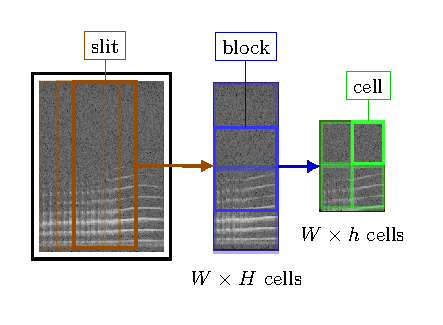
\includegraphics[width=0.7\textwidth]{image/slit_style_hog.pdf}
  \caption{Visualisation of the different areas defined in the slit style \gls{hog} transformation and how they are encapsulated in each other. The slit contains $4\times2$ cells and a block is $h=2$ cells high.}
  \label{fig:slit_style_hog}
\end{figure}

Summarized, the algorithm is described as follows: The spectrogram is windowed by a slit, a rectangle of size $x\times y$, the resulting slit images are then split up in $H\times W$ cells. These cells are then assigned to blocks, in such a way that the defined blocks overlap in the height by one cell, see \figref{slit_style_hog}. Per cell the gradients are extracted in $\pi$ bins, where the gradient bins are evenly spaced over 0 - 360 ("signed gradient"). The resulting gradient vectors are concatenated together per block in a vector with a size of $h\times W\times\pi$. The block vectors are then normalized and concatenated in the slit vector resulting in a size of $((H - h + 1)\times h)\times W\times\pi$ \cite{Terasawa2009}.

\section{Deep Learning}
We give a dense overview about \gls{dl} and the \glspl{ann} used in this project, for a full explanation see \cite{Goodfellow-et-al-2016,nielsen2015neural}.\\\\

\Gls{dl} is a further subdivision of ML, this specific learning type involves the use of \glspl{ann}.
Besides the existence of different learning strategies, we focused on supervised \gls{ml}.
It involves the manual labeling of data, which is then transformed into a dataset where the connection between subject and features is given. So the problem is to approximate a function (the target function) $f\colon X \to Y$ that maps the features from some domain X to the subject in some codomain Y.
As our goal is to distinguish multiple syllable types defining our classes, the features $X$ and the subjects $Y$ are vectors with the subject information being "one-hot" encoded. The "one-hot" encoding defines encoding by assigning the class to a position in a 1d vector where the vector for a subject has the value of one at the corresponding position and the other values are set to zero, see \figref{one-hot_encoding}.

\begin{figure}[ht!]
\centering
  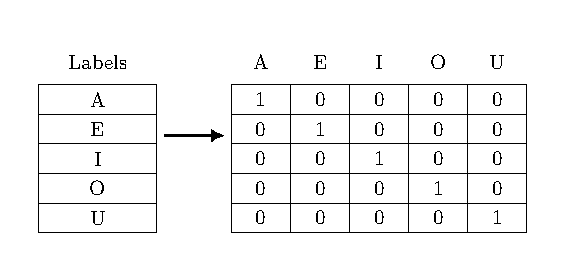
\includegraphics[width=0.7\textwidth]{image/one-hot_encoding.pdf}\hfill
  \caption{The "one-hot" encoding, the labels are replaced by a sparse feature vector, only the value at the corresponding position is one.}
  \label{fig:one-hot_encoding}
\end{figure}

In our case, $f$ is the function that maps an ultrasound recording slice to a syllable class, with the \gls{ann} models defined as a approximate function $\hat{f}(x, \Theta)$ parameterized by a finite-dimensional vector $\Theta^n \in \mathbb{Z}$ with some fixed $n$. The learning objective can be expressed as searching the values of the parameters $\Theta$ in a way that leads to the best possible function approximation.
The function $\hat{f}$ defines our \gls{ann} models, which is a parametric method, are bound by a fixed order or type of operations and only the values of the parameters $\Theta$ are variable.

For complex networks, learning the optimal values of the parameters is not trivial and is generally worked out by defining a cost function and stochastic optimizer algorithm.
The cost function should be adapted to the type of $y$ (and therefore to the output of the model too) and measure the extent to which the parameterized function $\hat{f}(x, \Theta)$ deviates from the target function $f$ in regard to the features from the dataset.
A suitable cost function over all datapoints is the crossentropy defined in (\ref{math:crossetropy}) describing the crossentropy between the training data $y^n$ and the model distribution, which is equivalent to the negative log likelihood.
\begin{equation}
    C=-\frac{1}{n}\sum_i^n\left(y_i\ln{\hat{y}}+(1-y_i)\ln{(1-\hat{y}_i)}\right) \label{math:crossetropy}
\end{equation}
The convention is that $0\ln{0} = 0$ but $\hat{y}\ln{0} = \infty$ for $\hat{y} \neq 0$ makes the loss function perfect for binary classification tasks.
For our multi-class classification task we took the categorical crossentropy loss function, it is the sum over $C$ classes from the crossentropy between the "one-hot" encoded training data and one model prediction of the same length, where the model prediction is normalized by a prepended softmax layer.
$$
L(y,\hat{y}\mathit{\_softmax}) = -\sum_{c=1}^Cy_c\ln{\hat{y}\mathit{\_softmax}_c}
$$
The softmax function is introduced in the next section \ref{sec:ann}.

A basic stochastic optimizer used for \gls{dl} is the \gls{sgd} algorithm. This algorithm alters the model parameters by specific proportions in respect to the gradient value of the cost.
$$
\Theta := \Theta - \eta\nabla J(\Theta)
$$
The proportion is defined by the learning rate $\eta$, this hyperparameter should be carefully tuned as it affects time and quality of the solution it converges to. A more sophisticated type of optimizer is the \gls{adam} algorithm, which is the one we use for our experiments.
Compared to the \gls{sgd}, it provides an adaptive learning rate per parameter and uses moments of the stochastic gradients to calculate the resulting values. The moments lead to smaller changes in direction.
One can imagine a ball entering from one side at the top of a valley and rolling downwards.
Due to the built-in moment calculation, the ball rolls straight down the valley after some zigzag movements, as if some force tries to keep the ball in the middle of the valley.
How much the forces of the moments influence the direction is controlled by the hyperparametres beta1 and beta2, which are the exponential decay rate of the first and second moment estimates.
Although \gls{adam} is controlled by three hyperparameters: learning rate, beta1, beta2; it is often sufficient to set the learning rate and the other two can be left at the default value.
As the learning objective has not changed, we used the same parameters as the framework provided.

These two algorithms are used in conjunction with the backpropagation algorithm.
For explanation, let us first consider the forward pass algorithm, which describes the first part of the training.
The forward pass of a simple feedforward network with three layers can be described in a mathematically simplified way with the chain rule $f(x)=f^{(3)}(f^{(2)}(f^{(1)}(x)))$, this implies that each layer is described by a function $f^{(d)}$. The first derivative of this function can be written out using the chain rule as follows $\frac{\partial f}{\partial x}=f^{(3)'}(f^{(2)}(f^{(1)}(x))f^{(2)'}(f^{(1)}(x))f^{(1)'}(x)$. It can be seen that the gradient calculation involves some repetitive calculations, e.g. $f^{(1)}(x)$. Such results are calculated and cached during the forward pass, this concept of caching intermediate results is called dynamic programming.
Then for "learning" the parameters, the backpropagation algorithm populates the error computed by the loss function back to the input layer and solves the partial derivative $\frac{\partial C}{\partial p}$ layer-wise, which results in the parameter gradient in respect to the error. Subsequently, leveraged by the stochastic optimisation algorithm, the corresponding gradient is applied to each parameter.

\subsection{Artificial neural networks}\label{sec:ann}
The \gls{ann} functions by imitating the neural connections made in the biological brain and connected these in a network of nodes, forming multiple layers.
In the \gls{mlp} architecture nodes are called perceptrons or neurons and are the computational units. The parameterized scalar valued function takes a set of inputs $x_1,\hdots,x_n$ and transforms the values by some parameters to the output $y$. The basic parameters are the weights $w_1,\hdots,w_n$, one for every input and the bias value $b$, through them one controls what the neuron computes. The processed input is given to an activation function (transfer function) $\sigma$ which is commonly a threshold function.
\begin{equation}
    y=\sigma\left(b + \sum\limits_{i=1}^{n}{x_iw_i}\right) \label{math:neuron}
\end{equation}
The math in a neuron is defined in (\ref{math:neuron}), which is an affine transformation of the input fed into an activation function.

\begin{figure}[H]
\centering
  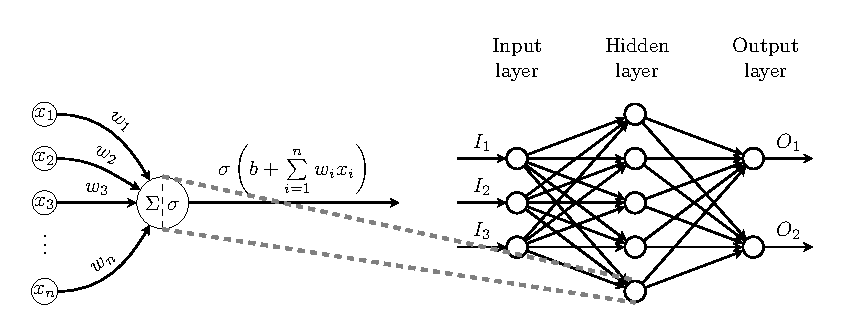
\includegraphics[width=0.9\textwidth]{image/mlp_schema.pdf}
  \caption{A diagram of a single perceptron, along with its position within a multilayer perceptron with fully connected layers.}
  \label{fig:mlp_schema}
\end{figure}
The \figref{mlp_schema} shows the structure of an \gls{mlp}, the neurons are stacked in layers, with sparse to fully connected neurons between the layers. The number of neurons per layer can vary and activation functions can normally change per layer. Basically, called as the "feedforward \gls{ann}", the layers are connected in an order, starting with the input layer which digests the provided features. This is then followed by one or more hidden layers, hidden because their activation is hidden from the outside, and in the end there is finally the output layer (a.k.a. classification layer). The output of a neuron is digested by the neurons of the next layer sequentially, thus the activations are only passed on to the subsequent layers.
This combination of neurons supports the aggregation of information from neurons specialised in the analysis of a single element to neurons at higher layers analysing more complex information.

The type of activation function and its respective abilities plays a crucial role for mapping complex functions, for example, a composition of linear functions is again a linear function, this implies that a \gls{mlp} with only linear functions as activation functions will decay into a single layer network handling linear tasks.
By selecting them consciously, they power the rise of the \gls{mlp} networks by granting them the ability to learn non linear boundaries.

\begin{figure}[ht!]
\centering
  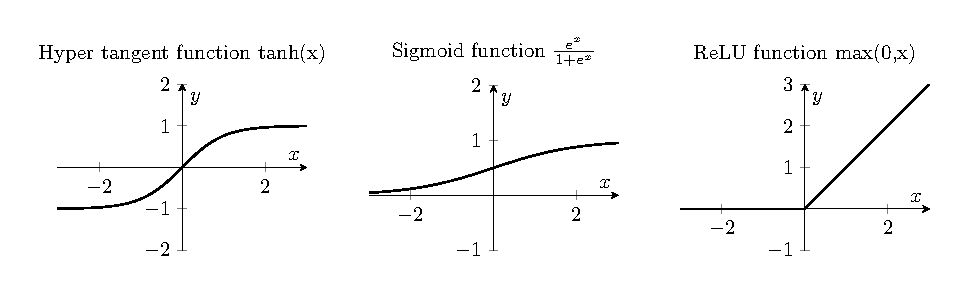
\includegraphics[width=0.7\textwidth]{image/activation_functions.pdf}\hfill
  \caption{Graphs of some activation functions used in ANN.}
  \label{fig:activation_functions}
\end{figure}

One of the first class of functions commonly used were sigmoidal functions such as the logistic function $\sigma(x)=\frac{e^x}{1+e^x}$ and the hyperbolic tangent function tanh. In recent years the computationally cheaper rectifier function $\sigma(x)=max(0,x)$ called rectified linear unit (ReLU) has become the most used function for deep neural networks \cite{Lecun2015}.
This function has the advantage over the sigmoid function, that the weights for large values do not become insignificant e.g. changing them influences the input in a linear manner as long it is over the threshold.
Because of this, the ReLU is seen as a possible approach to address the vanishing gradients problem when training deeper models.
For multi-class problems, the softmax function is commonly used for the output layer. The normalising exponential function is defined as $\sigma(x)_i = \frac{e^{x_i}}{\sum_{j=1}^C e^{x_j}}$ for $C$ classes, it is a generalization of the sigmoidal function for multiple dimensions. The calculated values can be seen as probabilities of how likely the network is to classify the input as one of the classes.

%
%Batch normalisation???? Goodfellow et al
%

\subsection{Long short term memory}
\Gls{lstm} architecture contains cells with a inherent state unit and the \gls{lstm} cells belong to the \gls{rnn}.\Glspl{rnn} are specialized networks to analyze sequence data. The \gls{rnn} cells hold a inner state, which influences the reception of the next value.
Because the basic \gls{rnn} cell does not control the alteration of the inner state, it tend to quickly "forget" information.
The \gls{lstm} cell, as the name implies, exhibits memory gates that control the values that update the internal state, which increases the memorization ability.

\begin{figure}[H]
\centering
  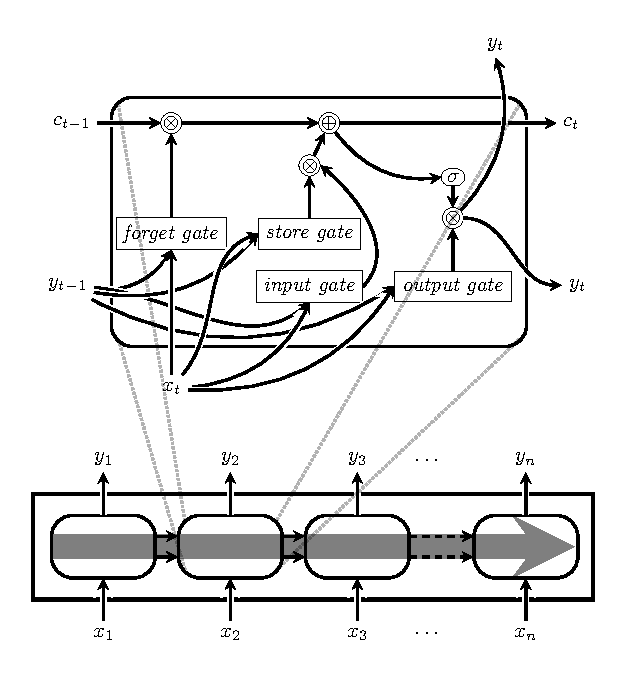
\includegraphics[width=0.7\textwidth]{image/lstm_schema.pdf}
  \caption{A diagram of a single \gls{lstm} cell and which values are recurrently used when processing a feature vector $x_1,\hdots,x_n$.}
  \label{fig:lstm_schema}
\end{figure}

The upper diagram of the \figref{lstm_schema} shows the inner parts of a typical \gls{lstm} cell. The previous output value and the new input value are both used by all gates to determine which part of the values should be changed.

The gates function by squeezing the values between 0 and 1 (usually the transformation function is a sigmoidal one), the resulting output is then multiplied point-wise by the destination vector, resulting in a down-regulation of some elements in the destination vector. The forget gate, for example, controls what is overwritten (what should be forgotten) in the state value. The input gate is a special case because it is the same function as the one used by the activation function.

The lower diagram exibits how the cell processes an input vector $x_1,\hdots,x_n$, where the current state $c_t$ and output $y_t$ is used for analyzing the next element. An elaborated and easily understandable description of the \gls{lstm} cell is provided by Christofer Ola on his blog \cite{Olah2015}.

\subsection{Convolution neural networks}
The \glspl{cnn} are a kind of deep neural networks tailored for image-like data and inspired by the behaviour of the animal visual cortex. They consist of convolution layers, containing a tensor of filters, where the values of the filters are the trainable parameters.
The filters are convolution kernels, a one or more dimensional matrix, which becomes convoluted over the input in a windowing manner.
% Similar the process can be adjusted by the padding and stride, depending on the configuration it leads to a bigger or smaller output.
The output of the convolution layer is then sent through an activation function.
\begin{figure}[H]
\centering
  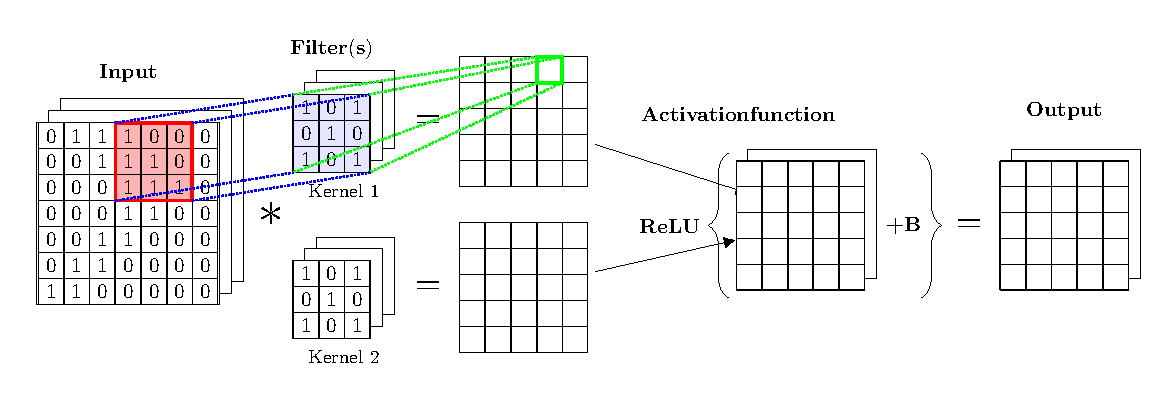
\includegraphics[width=0.7\textwidth]{image/cnn_schema.pdf}
  \caption{A diagram of a single convolution layer depicts the fate of the features through them.}
  \label{fig:cnn_schema}
\end{figure}

Overall, a convolution layer is entirely defined by four hyperparameters; the number of kernels $k$, their spatial extent $v$, the strides $s$ and padding $p$. Given an input of $[W_1, H_1, D_1]$, the corresponding convolution layer output $[W_2, H_2, D_2]$ relates to the input one as follows:
$$
W_2 = \frac{W_1-v-2p}{s+1}; \quad H_2=\frac{H_1-v-2p}{s+1}; \quad D_2 = k
$$
In our experiments we stick to the already implemented variants of hyperparameters v=3, s=1 and p=1 which seems to be a common choice \cite{Huang2017a, Simonyan2015}.

Compared to a layer in the \gls{mlp}, the neurons are quite similar, they are composed of weights, a bias and an activation function. The difference is, that the convolution neuron shares the activation function and only has a constrained set of weights per layer. This "constraint" allows the convolution layer to detect a characteristic, spatially local pattern in his receptive field, of the input data over the whole input at different places. Additionally, the stacking of convolution layers leads to non-linear filters that become responsive to larger regions of input space, so the networks creates representations of small parts (the receptive field) which are assembled to representations of larger areas.

\subsection{DenseNet}\label{sec:denseNet}
\begin{figure}[ht!]
\centering
  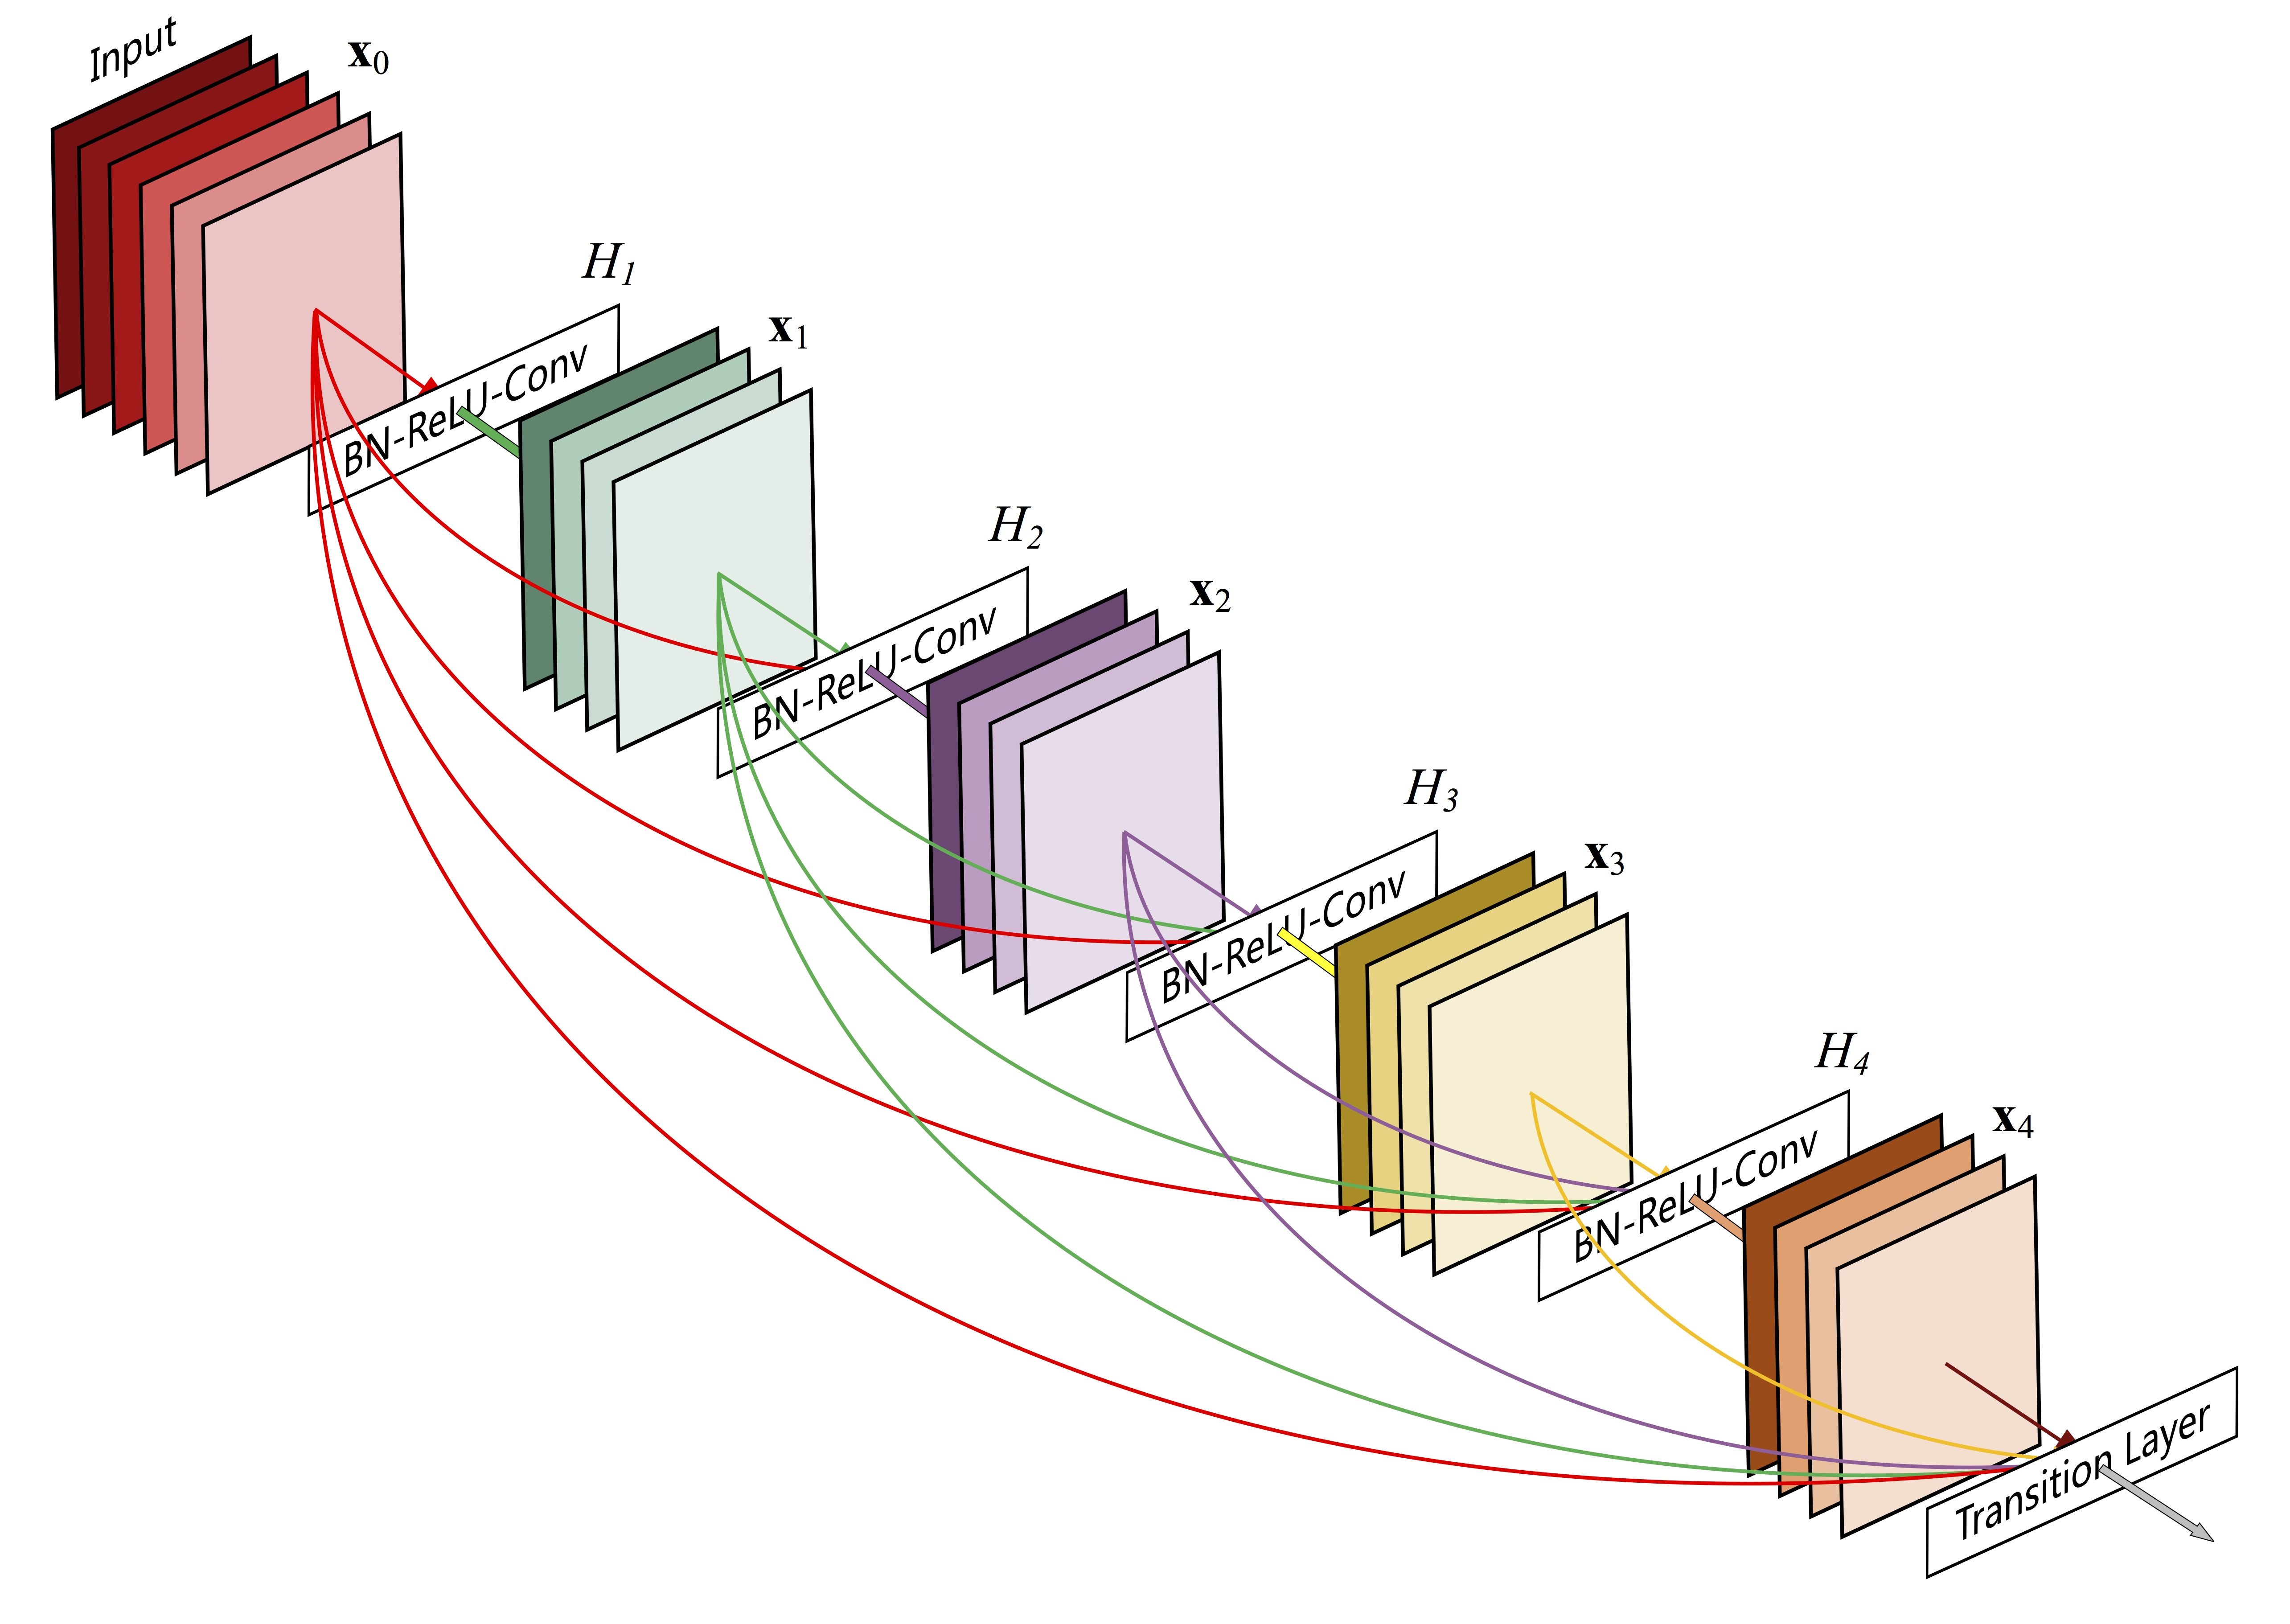
\includegraphics[width=0.5\textwidth]{image/denseNetBlock.jpg}
  \caption{Densely connected convolutional network block with 4 weight layers and a growth rate of 4. (© \cite{Huang2017a})}
  \label{fig:denseNet_block}
\end{figure}

The DenseNet takes advantage of the concept of additional connection by passing on layers, as other deep networks like ResNet. This idea stems from a problem which arises around deep networks; when continuously adding layers the performance saturates at some point. When adding more, e.g. increasing network depth beyond some point, it results in a significant drop in accuracy.
This concept of additional skip connections allows networks to be employed with more than 100 layers in a efficient manner.
In contrast to the skip connections from the ResNet, the DenseNet applies a dense connectivity pattern where the feature map of a layer $l$ is passed to all $L-l$ subsequent layers. This is worked out block-wise by concatenating the output of all previous layers as input to the next layer. Where a layer is a combination of convolution layers and max pooling.
As a direct consequence of the input concatenation, the feature maps learned by any of the
DenseNet layers can be accessed by all subsequent layers per block. This encourages feature reuse throughout the network, and leads to more compact models \cite{Huang2017a}.
Besides this, there are some evolving concepts incorporated, like bottleneck and full pre-activation \cite{He2016a}.
In addition, because of the skip connections, one can reduce the memory of the network with some nice tweaks like sharing the memory for outputs between the subsequent inputs in a dense block \cite{Huang}.


\subsection{Regularization}
The \gls{ann} network architecture used in the experiments constitutes a complex computational model, which incorporates a high number of parameters. With the limited data we have, this makes the network prone to overfitting. Fortunately, the field of \gls{ann} has an arsenal of regularization techniques to prevent overfitting, we present the ones used in our models.

% https://link.springer.com/article/10.1007/s11042-019-08453-9
With Dropout, the \gls{ml} model randomly drops units from the network during training, which corresponds to an activation of zero \cite{Srivastava2014Dropout:Overfitting}. For every training example digested by the network the input or neurons are randomly dropped with probability $p$ resulting in a thinned input and a thinned network. This forces the model to create alternate decision paths and hopefully simpler ones. The backpropagation of the training step then only concerns the parameters of the thinned network (respectively the retained neurons and inputs), which leads to the training of an ensemble of thinned networks. After a training step, when evaluating the model on the validation set, the full model without dropout is used. To account for the scaled weights of the neurons to which dropout is applied, the weights are multiplied by the probability $r=1-p$, i.e. the probability that they are retained in the network. This should grant that for any involved neurons the expected output at training time should be equally to the output at test time \cite{Srivastava2014Dropout:Overfitting}.

Max pooling has some regularization abilities, but this is not the main focus of this concept.
The pooling layer is commonly combined with a convolution layer at the front and it subsamples its input tensors into a smaller output tensor. The subsampling is applied to every channel, therefore the resulting tensors only vary in width and height where the channel stays the same. The subsampling is done in a sliding window manner where the values of a window are sampled in respect to the pooling operation. Common pooling operations are max, average or $L^2$-norm and common hyperparameters are $2\times2$ for patch size and strides.
One advantage of applying a pooling layer to a feature layer is that the features are invariant to small spatial shifts. This can be useful when detecting the presence of a pattern is more important than determining its exact position. Unfortunately, this nice feature leads to the loss of some information in the layer.

\section{Evaluation}
\Gls{ann} can be difficult to understand, as their inner workings become, in a way, obfuscated by the large number of units. Compared to SVM or other similar \gls{ml} models it could be near to impossible to explain the effect of a unit on the network, e.g. knowing which changes of the hyperparameters leads to which exact outcome.
Therefore, we use tools for evaluating the models in a way that we can understand the inner working in a broader view. In this chapter we will introduce some methods to train and evaluate \gls{ann} models.

\subsection{K-fold cross-validation}
%https://stats.stackexchange.com/questions/27730/choice-of-k-in-k-fold-cross-validation
%https://stats.stackexchange.com/questions/61783/bias-and-variance-in-leave-one-out-vs-k-fold-cross-validation?answertab=votes#tab-top

A model validation method is used for measuring the extent to which a model generalizes, e.g. how good it performs on unseen data.
The generalisation can be assessed by comparing the predictions from the unseen data with the true output.\\\\

K-fold \gls{cv} is a model validation method and is a general tool for selecting models on datasets with difficult-to-check assumptions on the data generating process \cite{Zhang2015}.
It is preferred over other methods when the dataset has limited samples, as it run the model on the whole data, with the trade-off that multiple runs are conducted per dataset and \gls{ml} model.
As the name of the method already implies, the experiment is executed $k$ times.
The data is evenly spread over $k$ bins, with the shortest classes defining the bin size. The remaining samples are added to the training set.
In every round the model is trained on $k-v-t$ bins plus the remaining samples, where $v$ is the number of validation bins and $t$ is the number of testing bins used. After each run, the bins are shifted by one, so that all subsets contain every bin at least once.
\begin{figure}[H]
\centering
  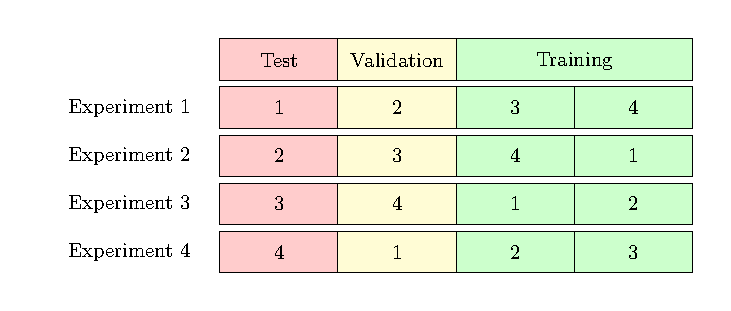
\includegraphics[width=0.7\textwidth]{image/k-fold_cv.pdf}
  \caption{A visualisation of the distribution of bins in a k-fold \gls{cv} with $k=4$, using one bin each for validation and testing.}
  \label{fig:k-fold_cv}
\end{figure}
In the context of this method we speak about two different estimations made on unseen data. One is during model maturation where the unseen data belonging to the validation set is used for picking the model in the best state. The other (belonging to testing) provides a fair assessment on the maturated model, after the test, no changes on the (hyper)parameters should be made anymore.

% https://link.springer.com/chapter/10.1007%2F978-3-319-44636-3_4
An additional input about model generalisation is provide by Juan Gabriel Colonna et al. \cite{Colonna2016}.
They propose to include the species and specimen information at the split process in a way, that syllables of one specimen are in test or validation only. This enables the assessment of how well the model is generalized for detecting syllables of new specimen of the same species. As we are interested in the performance on different feature presentations, we omitted this kind of preparation. In a future work, the integration of species and specimen information would become interesting!

% mit andreas besprechen

In our experiments, the samples were stratified by their labels and then distributed evenly to the bins depending on their input order, in contrast to the basic concept where the samples are distributed in a randomized manner. We chose this concept because it ensures that samples of the same audio are more likely in the same bin than distributed over all bins, which should result in a more accurate estimation on how the model could generalize as the validation and test bins are less likely to contain a sample of the same audio as a sample exiting in the training bins.
However, due to this decision, we loose the nice feature of randomization, which helps to break preexisting order of datapoints and ensures a similar distribution as possible.

\subsection{Learning curves}
% https://www.baeldung.com/cs/learning-curve-ml
We already showed how the training is done in this project, but how do we assess this? And how is this used to select the interesting model, i.e. parameter set?\\\\

During the training phase of a model one can monitor the loss and accuracy of the \gls{ml} model on the training set and the validation set. The resulting visualisation graphs of loss or accuracy over time belong to the learning curves, they are widely used as diagnostic tools for \glspl{ann}, as they learn from the data set in an incremental manner.

The training curves provide information about how well and quickly the model can learn from the data.
If the model is too simple (e.g. small \gls{ann}) the model tends to struggle with the learning data, called underfitting. As the model is unable to capture the patterns in the training data, the accuracy plateaus at low magnitude and the loss remains relatively high.

\begin{figure}[ht!]
\centering
  \includesvg[inkscapelatex=false,width=0.9\textwidth]{image/generated/train_val_cnn_1d_sct_compressed_nrs0_raw_100.svg}\hfill
  \caption{Visualisation of the training curves exibiting overfitting, with the accuracy and loss curves merged into one plot. The validation loss draws a U-shaped curve with a increasing gap to the training loss and the training accuracy is about 10\% higher than the validation accuracy.}
  \label{fig:train_val_cnn_1d_sct_compressed_nrs0_raw_100}
\end{figure}

By considering all four graphs, one can extract information about overfitting and how the validation data is represented by the testing data and vice versa.
Overfitting becomes visible by plotting both accuracy graphs together. Where over time the gap between the greater training accuracy and lower validation accuracy becomes visible.
Commonly, this gap increases over time, as the model starts to over optimize more and more to fit to the training data.
The overfitting behaviour is also visible when comparing the two loss curves, with the training loss curve getting steadily lower and the validation loss curve initially decreasing until it starts to increase, sometimes exponentially, resulting in the typical U-shaped curve.

Consider an accuracy and loss graph from the validation data, one option would be to select the epoch with the lowest loss value, but as we are more interested in the accuracy and the loss value is typically only used as a proxy for the accuracy, the better choice is to select the model where the validation accuracy stops improving. But when does accuracy stop improving? One can say this happens when the accuracy starts to plateau the first time or starts fluctuating around the same value for some epochs. It could happen that if we train over many more epochs after the accuracy starts to plateau, that it increases again, but the magnitude would likely be small and therefore be negligible \cite{nielsen2015neural}.
As this seems to be a valid point, there exists a different view; Goodfellow et al. suggest in the book deep learning \cite{Goodfellow-et-al-2016} to select the model with the lowest validation loss, as the generalization is then typically maximized.

Therefore, we tend to take one snapshot of the epoch with the lowest validation loss and one with the highest validation accuracy. Finally, in the results, we stick to the second metric because of our interest in comparing the accuracy.

% andreas

\subsection{Layer wise relevance propagation}\label{sec:evaluation_lrp}
% https://towardsdatascience.com/indepth-layer-wise-relevance-propagation-340f95deb1ea
% https://git.tu-berlin.de/gmontavon/lrp-tutorial
% https://lrpserver.hhi.fraunhofer.de/

For image-like features, there is a well-suited technique called \gls{lrp}.
After a forward pass, the algorithm searches neurons that contribute most to the result backwards through the network.
This is done by examining the weights and activations from the forward pass. The contribution of a neuron is significant if it has a high activation value and it contributes to a lot to relevant neurons in the deeper layers.
The result can then be visualised as a heat map where the areas with high pixel values are the most important for getting a certain result.
Unfortunately, the python framework ”innvestigate” used to explore the \gls{dl} model was not fully supported by the TensorFlow version used.
Therefore some changes were made with insufficient knowledge about the code of the framework in question, in the hope that they would have limited damage on the results. Thus, when interpreting the results they should be taken with a pinch of salt.
